% Fair topics for CS340 MIDTERM:
% \begin{enumerate}
%     \item test vs. training
%     \item decision trees
%     \item decision stumps
%     \item naive Bayes
%     \item k-nn
%     \item ensemble methods
%     \item clustering
%     \item outlier detection
%     \item least squares
%     \item norms
%     \item change of bases (polynomial bases)
%     \item log-sum-exp
%     \item huber
%     \item gradient descent
%     \item linear 
%     \item nearest neighbors
%     \item k-means clustering
%     \item naive Bayes
%     \item Probabilistic classification
%     \item cross validation
% \end{enumerate}

\documentclass{article}

\usepackage{fullpage}
\usepackage{color}
\usepackage{amsmath}
\usepackage{url}
\usepackage{verbatim}
\usepackage{graphicx}
\usepackage{parskip}
\usepackage{amssymb}
\usepackage{amsfonts}
\usepackage{nicefrac}
\usepackage{listings} % For displaying code
\usepackage{algorithm2e} % pseudo-code
\usepackage{natbib}
\usepackage{todonotes}
\usepackage{caption}
\usepackage{subcaption}
% Answers
\def\rubric#1{\gre{Rubric: \{#1\}}}{}
\def\ans#1{\par\gre{Answer: #1}}
% Colors
\definecolor{blu}{rgb}{0,0,1}
\def\blu#1{{\color{blu}#1}}
\definecolor{gre}{rgb}{0,.5,0}
\def\gre#1{{\color{gre}#1}}
\definecolor{red}{rgb}{1,0,0}
\def\red#1{{\color{red}#1}}
\def\norm#1{\|#1\|}
\usepackage{xcolor}
\usepackage{listings}


\definecolor{codegreen}{rgb}{0,0.6,0}
\definecolor{codegray}{rgb}{0.5,0.5,0.5}
\definecolor{codepurple}{rgb}{0.58,0,0.82}
\definecolor{backcolour}{rgb}{0.95,0.95,0.92}

\lstdefinestyle{mystyle}{
    backgroundcolor=\color{backcolour},   
    commentstyle=\color{codegreen},
    keywordstyle=\color{magenta},
    numberstyle=\tiny\color{codegray},
    stringstyle=\color{codepurple},
    basicstyle=\ttfamily\footnotesize,
    breakatwhitespace=false,         
    breaklines=true,                 
    captionpos=b,                    
    keepspaces=true,                 
    numbers=left,                    
    numbersep=5pt,                  
    showspaces=false,                
    showstringspaces=false,
    showtabs=false,                  
    tabsize=2
}

\lstset{style=mystyle}
% Math
\def\R{\mathbb{R}}
\def\argmax{\mathop{\rm arg\,max}}
\def\argmin{\mathop{\rm arg\,min}}
\newcommand{\mat}[1]{\begin{bmatrix}#1\end{bmatrix}}
\newcommand{\alignStar}[1]{\begin{align*}#1\end{align*}}
\def\half{\frac 1 2}

% LaTeX
\newcommand{\fig}[2]{\includegraphics[width=#1\textwidth]{#2}}
\newcommand{\centerfig}[2]{\begin{center}\includegraphics[width=#1\textwidth]{#2}\end{center}}
\def\items#1{\begin{itemize}#1\end{itemize}}
\def\enum#1{\begin{enumerate}#1\end{enumerate}}

\begin{document}

\title{CPSC 340 Machine Learning Take-Home Midterm Exam\\ (Fall 2020)}


\section*{Question 2}
\setcounter{section}{0}

\section{Team}
\begin{tabular}{|c | c | c |} 
\hline
Team Members & \emph{Shuyang Ye} & \emph{Ning Shen} \\
\hline
Student ID & \emph{96481163} & \emph{70533633} \\
\hline
CS ID & \emph{l8n8s} & \emph{i0c1p} \\
\hline
\end{tabular}
\begin{tabular}{|c | c |} 
\hline
Kaggle Team Name & \emph{123321}\\
\hline
\end{tabular}
\section{Solution Summary}
    To predict the future path of ego cars, we first decide which machine learning model to be adopted. Considering the training set only cover the track from last 1 second, and the task is to predict 3 second forward, AR model is not suitable. On the other hand, KNN is a good choice. We just need to find the similar cases. Here, ``similar'' means the tracks in last 1 second are close enough in regard to Uclidean distance. ``Others'' cars and ``agent'' car are considered seperately. First, we calculated the similarity of ``others'' between training set intersection and test set intersection. Second, we calculated the similarity betweem ``agent'' cars. Then, we pick k nearest intersections(examples) based on the overall distance and average the corresponding ``agent'' car's track in 3 second to be our prediction. \\
    Hyperparameters are the $k$ from KNN and a weight $w$ which is used to balance the influence from ``others'' and ``agent''. We use validation set finding that k=6 and w=1 can yield best validation error. To conclude, in our model, comparing ``agent'' car is adequate for predicting the future track.
\section{Experiments}
    The main experiment is to find the best hyperparameters. As we explained in the Summary, the similarity between two intersections comes from two different sources: ``others'' and ``agent''. During the comparison, we realize ``agent'' must pair with ``agent'', ``others'' pairs with ``others''. For ``others'', we establish the distance matrix of size 9*9. Each element $d_{ij}$ is the distance between the track of $\textnormal{car}_i$ from intersection 1 and of $\text{car}_j$ from intersection 2. For the intersection with less than 9 ``others'', the corresponding $d_{ij}$ will be filled with np.inf. Once the distance matrix is completed, we apply the greedy search algorithm to find the similarity. We first find the smallest $d_{ij}$ in the matrix, which means $\textnormal{car}_i$ and $\textnormal{car}_j$ are paired. Then we delete row i and column j and search for the smallest $d_{i'j'}$ from the new matrix. Repeating above steps until there is no available $d_{ij}$. Averaging all the $d_{ij}$ found yields the similarity ($s_1$) of ``others''. For ``agent'' part, we directly compute Uclidean distance between two ``agent'' cars ($s_2$). The total similarity is weighted by w: $s = (1-w)*s_1+w*s_2$. For each example from validation set, we sort the total similarity $s$ to find k nearest neighbors, in other word, k most similar intersections from training set. The averaged $y$ from these intersection is the predicted track $y_{\textnormal{pred}}$. The validation error is evaluated by the different between $y_{\textnormal{pred}}$ and $y_{\textnormal{val}}$. Figure 1 shows how does the hyperparameters impact the validation error.
    \begin{figure}[h]
        \centering
        \begin{subfigure}[h]{0.6\textwidth}
            \centering
            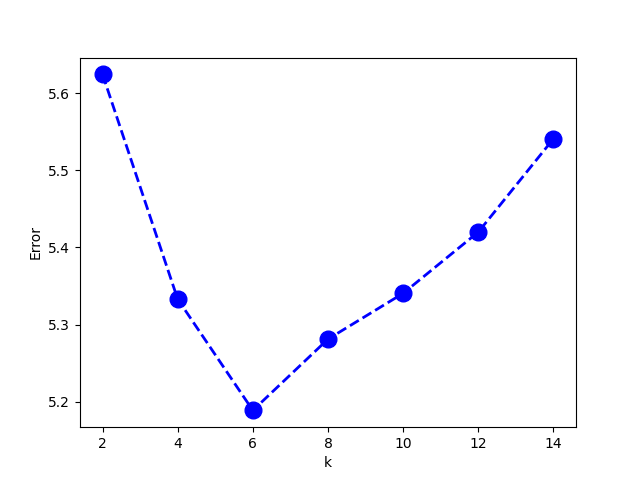
\includegraphics[width=\textwidth]{../figs/scan_k.png}
            \caption{$\textnormal{Error vs k(w=1)}$}
            \label{Error vs k}
        \end{subfigure}
        \hfill
        \begin{subfigure}[h]{0.6\textwidth}
            \centering
            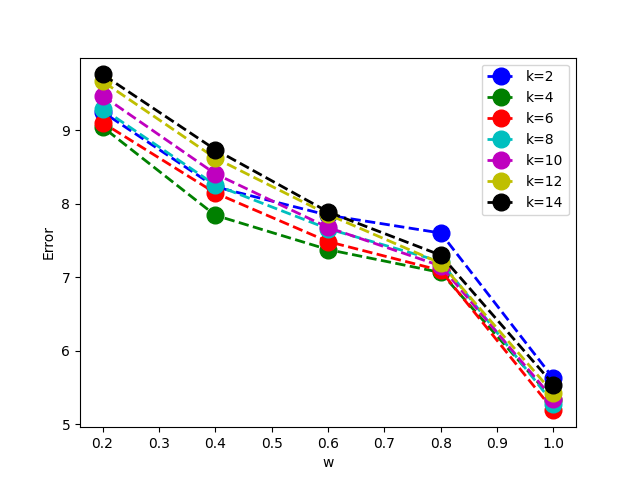
\includegraphics[width=\textwidth]{../figs/scan_w.png}
            \caption{$\textnormal{Error vs w}$}
            \label{Error vs w}
        \end{subfigure}
        \caption{hyperparameters scan}
        \label{Hyperparameters scan}
   \end{figure}\\
   The experiment result reveals the fact that there is no need to include ``others'' into the similarity. Thus, we have done the feature selection: only the data of ``agent'' car is selected. 
\section{Result}
    \begin{center}
        \begin{tabular}{|c | c |} 
        \hline
        Team name & Score \\ [0.5ex]
        \hline\hline
        123321 &  0.54513\\
        \hline 
        \end{tabular}
    \end{center}
\section{Conclusion}
    We used KNN as our model. An experiment of hyperparameters choosing is done which also help us to select feature. We found similar ``agent'' cars tend to have the close track in 3 second.


\end{document}